% This is samplepaper.tex, a sample chapter demonstrating the
% LLNCS macro package for Springer Computer Science proceedings;
% Version 2.20 of 2017/10/04
%
\documentclass[runningheads]{llncs}
\usepackage{graphicx}
\usepackage{amsmath}
\usepackage{multirow}

\begin{document}
%
\title{Scattering Convolutional Networks for Image Classification and Analysis}
%
%
\author{Quentin Le Roux}
%
%
\institute{Université Côte d'Azur, France}
%
\maketitle              % typeset the header of the contribution
%
\begin{abstract}
A scattering network is a cascade of wavelet transforms with non-linearities. They produce invariants: feature maps invariant to rotation, translation, and small deformations. Comparable to convolutional neural networks, they can surpass them in areas such small dataset classification while displaying mathematical certainty and explanability. This report broadly covers their concept and most recent developments.
%
\keywords{Wavelet \and Wavelet Transforms \and Scattering Networks \and Convolutional Neural Networks}
\end{abstract}
%
\section{Signal Decomposition}

\subsection{Origins: the Fourier Transform}

\subsubsection{The Fourier Transform} (FT) extracts frequency and amplitude information from stationary signals but obfuscates frequency-time information.
\begin{align}
    \hat{f}(\omega)&=\underset{-\infty}{\overset{+\infty}{\int}}f(t)e^{-2\pi i \omega t}dt\\
    t&,\,\text{time};\,\,\omega,\,\text{a frequency};\,\,f(t),\,\text{a signal intensity vs. time function}\notag
\end{align}

\subsubsection{The Short-Time Fourier Transform} (STFT) helps deal with non-stationary signals. It extracts localized frequency information in a given time window, relying on the assumption that a non-stationary signal still presents stationary windows. This results in computing FT for fixed-length slices of a signal.
\begin{align}
    \hat{f}(\omega, \tau)&=\underset{-\infty}{\overset{+\infty}{\int}}f(t)w(t-\tau)e^{-2\pi i \omega t}dt\\
    w&,\,\text{a window function};\,\,\tau,\,\text{a translation parameter}\notag
\end{align}

Fixed-length time windows result in interfering frequency and time resolutions, however. Short windows are best suited for high frequencies (effective time but poor frequency resolutions) while wide windows are best suited for low frequencies (effective frequency but poor time resolutions).

\subsection{Wavelets}

Wavelets are small, localized wave-like functions\cite{andrew_nicoll}. Parametrized by two factors, window size, and scaling (the width and mean frequency -- larger scaling yields better frequency resolution and shorter scaling better time resolution), they help solve STFT's time-frequency trade-off.
\begin{align}
    \hat{f}(s, \tau)&=\frac{1}{\sqrt{|s|}}\underset{-\infty}{\overset{+\infty}{\int}}f(t)\psi(\frac{t-\tau}{s})dt\\
    \psi&,\,\text{a wavelet function};\,\,s=\frac{1}{f},\,\text{the scale};\,\,\tau,\,\text{the window size}\notag
\end{align}

\section{From Wavelets to Scattering Networks}

\subsection{The importance of invariance in signal analysis}

Invariance implies reducing signals' intra-class variability, i.e. constructing invariants to translation and transposition (audio), rotations and scaling (images). 
\begin{align}
    \forall c\in\mathbb{R}&,\,\,x_c(t) = x(t-c)&\text{(translation)}\\
    \forall \tau, x_\tau(t) &= x(t-\tau(t))&\text{(deformation)}
\end{align}

Invariance was further described as a Lipschitz continuity condition\cite{bruna2012invariant}\cite{mallatlecture}:
\begin{align}
    ||\Phi(x_\tau)-\Phi(x)||&\le C\,\underset{t}{sup}\,|\nabla\tai(t)|.||x||&\text{($\underset{t}{sup}\,|\nabla\tau(t)|$, the deformation size)}
\end{align}

Invariance to translation and deformation is key in signal analysis, especially classification as signals are often characterized by non-rigid deformations resulting in high intra-class variance\cite{bajcsy}\cite{keysers}\cite{trouve}.

It has been shown that FT are only robust to small deformations\cite{bruna2012invariant}. They erase high frequencies and thus are not suitable for building robust invariants. With their localized characteristic, wavelets help build invariance, albeit imperfectly, to both translation and deformation compared of FT\cite{bruna2012invariant}\cite{mallatlecture}.

\subsection{Discrete Wavelet Transform and multilevel decomposition}

Computing wavelet coefficients $\hat{f}(s,\tau)$ at every scale and window is inefficient. This is solved by the Discrete Wavelet Transform (DWT):
\begin{align}
    \hat{f}(s, \tau)&=\frac{1}{\sqrt{|s|}}\underset{m=0}{\overset{p-1}{\sum}}f(t_m)\psi(\frac{t_m-\tau}{s})\\
    s&=2^{-j}\,\,\text{the dyadic dilation}\notag;\,\,\tau=k2^{-j}\,\,\text{the dyadic position}\notag\\
    j&,\,\,\text{the scale index};\,\,k,\,\,\text{the wavelet transform signal index}\notag
\end{align}

The DWT ends up providing a comparatively finer signal windowing and time-frequency trade-off (See Fig.~\ref{fig1}).
\begin{figure}
\centering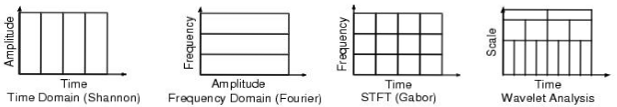
\includegraphics[width=\textwidth]{dwt.png}
\caption{DWT allow efficient retrieval of low and high frequency information\cite{dwt}.} \label{fig1}
\end{figure}

\subsection{Wavelet Transforms}

Wavelet Transforms (WT) solve the high frequency issue of previous feature mapping methods such as the Scale-invariant Feature Transform (SIFT)\cite{bruna2012invariant}. These prior methods usually build a lower-dimensional manifold first followed by a task-dependent supervised or unsupervised method, e.g. Support Vector Machines (SVM), Gaussian Mixture Models (GMM)\cite{sanchez1}\cite{sanchez2}.

WT are obtained by duplicating (via rotation and dilation) and convolving a wavelet function $\psi_\lambda(t)$ to cover the entire frequency domain of a signal. WT are the resulting set $W_x(t)$ of convolutions $x\star\psi_\lambda(t)$ of an input signal $x$ such that the lowest frequencies are recorded via a low pass filter $\phi$\cite{mallatlecture}:
\begin{align}
W_x(t)&=\big\{x\star\phi, x\star\psi_\lambda(t)\big\}_\lambda\\
\lambda&,\,\,\text{a rotation tuning parameter}\notag
\end{align}

WT are not translation-invariant per se due to an averaging-in-time operation at high frequencies that induces a loss of information in order to build invariants.

\subsection{Scattering Transforms}

WT's loss of information is addressed by introducing the non-linear modulus operator, and an iterative process relying on a function $U_x$ called a scattering propagator\cite{bruna2012invariant}\cite{mallatlecture}:
\begin{align}
U_x(t)&=\big\{x\star\phi, |x\star\psi_\lambda(t)|\big\}_\lambda\\
\forall z \in \mathbb{C},\,\, z &= a + ib\notag\\
|z|&=\sqrt{a^2+b^2}\notag
\end{align}

A Scattering Transform (ST) is the result of an accumulated composition of scattering propagators $U_x$, yielding intermediary output $x\star\phi$ at each composition step, and passing $|x\star\psi_\lambda(t)|$ as input to the next composed propagator, resulting in a path $S$ constructed over all rotations $\lambda$ of the underlying WT (See Fig.~\ref{fig2}).
\begin{align}
\forall\text{ path }p&=(\lambda_1, ..., \lambda_m)\,\text{ of order $m$}\notag\\
S[p]x(t) &= ||\hdots||x\star\psi_{\lambda_1}|\star\psi_{\lambda_2}|\hdots|\star\psi_{\lambda_m}|\star\phi
\end{align}

This results into a tree $S$ parametrized by a scale $J$ and $L$ different orientations for the underlying wavelet functions\cite{oyallon}. Of order 1 (i.e. $m=1$), ST are similar to SIFT\cite{lowe}. Furthermore, it has been shown that branches (i.e. paths) of the ST tree $S$ can be intelligently pruned to accelerate computation -- interesting features are concentrated along specific paths of the tree $S$ such that the ST requires $\mathcal{O}(n\,\,log\,\,n)$ operations \cite{bruna2012invariant}\cite{oyallon}.
\begin{figure}
\centering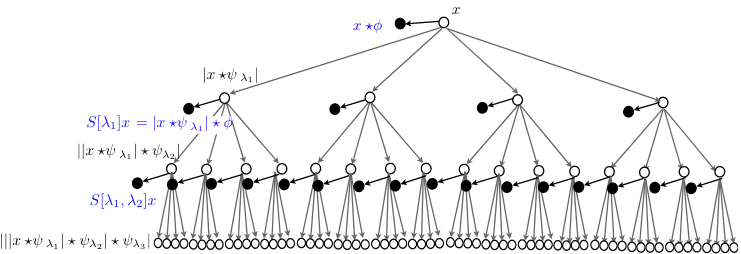
\includegraphics[width=\textwidth]{graph_rep.png}
\caption{Graphical representation of a ST of order 3\cite{mallatlecture}.} \label{fig2}
\end{figure}
Such a tree computation (simultaneous feature propagation and low-pass filtering\cite{DSN}) results in a deformation, rotation and translation-invariant feature representations of a given signal \cite{mallatgroup}\cite{mallatIEEE}\cite{mallatlecture}. Those mappings happen to be sparse, accurate, and stable representations with relatively few parameters\cite{bruna2012invariant}.

\subsection{Scattering Networks}

ST were pioneered by Joan Bruna and Stéphane Mallat in 2012 after classical convolutional neural network (CNN) architectures rose from relative obscurity around 2010\cite{lecun}. ST have simultaneously been described as Scattering Networks (SN) and a non-learned wavelet-cascade approach comparable to CNN\footnote{"The scattering transform is defined as a complex-valued convolutional neural network whose filters are fixed [...] and the non-linearity is a complex modulus. Each layer is a wavelet transform, which separates the scales of the incoming signal. [...] The result is a reduction of variance and a stability to additive noise\cite{andreux}."}\cite{bruna2012invariant}\cite{mallatIEEE}\cite{mallatlecture}\cite{DSN}.

Scattering networks hyper-parameters are dimension-dependent\cite{andreux}\cite{mallatgroup}\cite{mallatIEEE}\cite{mallatlecture} as they characterize their output shape, see Table~\ref{tab1}. The input of a 1-dimensional ST is of shape $(T)$ where $T$ the length of the signal. Its output is of shape $(P, \frac{T}{2^J})$, with $P \propto 1+JQ + J(J-1)\frac{Q}{2}$ the number of scattering coefficients\cite{anden}. The input of a 2-dimensional ST is of shape $(C, W, H)$ where $C$ is the number of channels, and $W$ and $H$ are respectively the width and height of the signal. Its output is of shape $(C, 1+LJ + \frac{L^2J(J-1)}{2},\frac{W}{2^J},\frac{H}{2^J})$\cite{bruna2012invariant}. The output of a scattering network of order $m=2$ on an entry from the MNIST dataset\cite{lecun2} is reproduced in Fig.~\ref{fig2}.
\begin{table}\centering
\caption{Hyperparameters for 1- and 2-dimensional SN}\label{tab1}
\begin{tabular}{| p{2cm} | p{2.5cm} | p{7cm} |}
\hline
Hyperparam. & ST dimension & Explanation \\
\hline
$\quad J$ & 1D, 2D & The number of scales to cover the input signal \\
$\quad Q$ & 2D & The number of wavelets per octave \\
$\quad L$ & 2D & The number of angles to cover the input signal \\
\hline
\end{tabular}
\end{table}

Paired with a SVM or a PCA, SN were found to outperform CNN on texture discrimination tasks, only necessitating to be of order 2\cite{mallatIEEE}\cite{mallatlecture} (a higher $m$ only yields marginal error reductions). Furthermore, they were found to be more robust than other methods, especially with subsampled datasets (see Table~\ref{tab2}).
\begin{figure}
\centering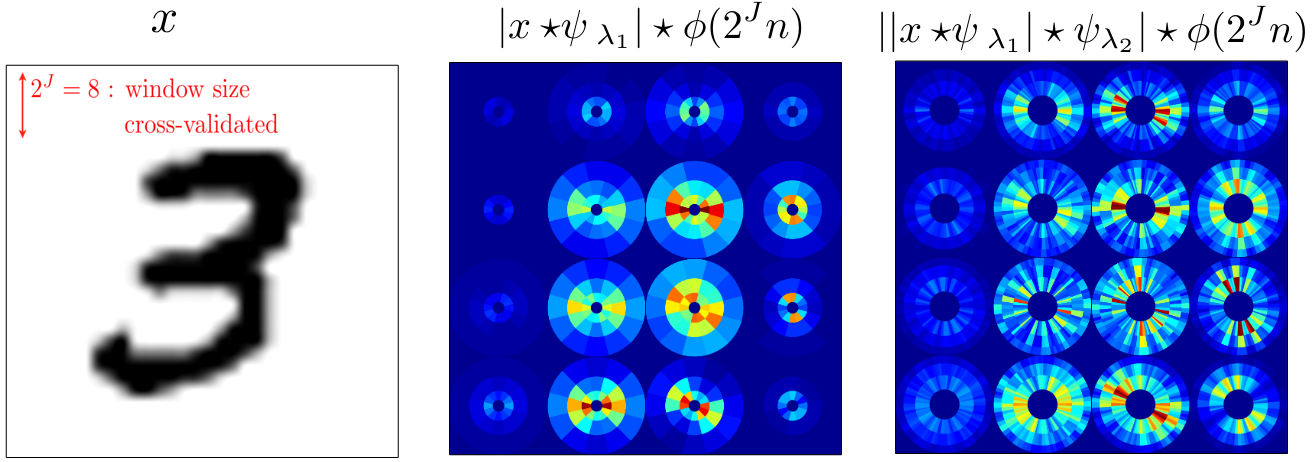
\includegraphics[width=\textwidth]{MNIST.png}
\caption{SN output ($m=2$, $J=3$, and $L=12$) on a MNIST dataset entry \cite{maison}\cite{mallatlecture}.} \label{fig2}
\end{figure}

Most state-of-the-art implementations before 2018 applied to texture discrimination databases\cite{textureKTH}\cite{textureUIC}\cite{textureUMD} and the MNIST, as it was noted at inception that more complex datasets like Caltech101\cite{caltech} display complex variabilities where learned approach would be more suited\cite{bruna2012invariant}.
\begin{table}\centering
\caption{Classification error of a SN against a then state-of-the-art CNN\cite{lecun} on the MNIST dataset, reproduced from \cite{bruna2012invariant}.}\label{tab2}
\begin{tabular}{| p{2cm} | p{1cm} | p{1cm} | p{3.2cm} | p{3.2cm} | p{1cm} |}
\hline
Training Size & PCA & SVM & SN with PCA ($m=2$) & SN with SVM ($m=2$) & CNN \\
\hline
300 & 14.5 & 15.4 & \textbf{4.7} & 5.6 & 7.18 \\
1000 & 7.2 & 8.2 & \textbf{2.3} & 2.6 & 3.21 \\
2000 & 5.8 & 6.5 & \textbf{1.3} & 1.4 & 2.53 \\
5000 & 4.9 & 4 & \textbf{1.03} & 1.4 & 1.52 \\
10000 & 4.55 & 3.11 & 0.88 & 1 & \textbf{0.85} \\
20000 & 4.25 & 2.2 & 0.79 & \textbf{0.58} & 0.76 \\
40000 & 4.1 & 1.7 & 0.74 & \textbf{0.53} & 0.65 \\
50000 & 4.3 & 1.4 & 0.7 & \textbf{0.43} & 0.53 \\
\hline
\end{tabular}
\end{table}

\section{State-of-the-Art Applications of Scattering Networks}

\subsection{Hybrid Networks}

Given that the first layers in learned CNN are similar to WT\cite{mallatlecture}, hybrid networks (HN, where the first learned layers of a neural network are replaced by a fixed SN) were first proposed in 2012\cite{bruna2012invariant} then implemented in 2018\cite{oyallon}. One of the main advantages of HN is the production of non-learned local encodings that reduce the number of learned parameters in a network, allowing for faster and lighter learning with only marginal increase in error rates, while also being robust to subsampling of datasets. HN (with either fully-connected layers or CNN) were found to rival learned methods\cite{oyallon} for classification and unsupervised feature representations on the STL-10\cite{stl}, ImageNet\cite{imagenet}, and CIFAR-10\cite{cifar} datasets.

\subsection{Max-Pooling layer variant}

An extension to HN, scattering-maxp networks (SMPN) were recently introduced\cite{DSN}. SMPN relies on a continuous max-pooling as a non-linearity at the scattering propagator level to reduce the final amount of learned-parameters (up to 8-fold reductions with standard HN and 12-fold with fully-learned CNN like VGG-16 \cite{vgg}) while retaining translation invariance with only marginal performance reduction (tested on the Caltech101 and Caltech256\cite{caltech256} datasets).

\subsection{Image reconstruction and generation}

It has been supposed\cite{brunathesis}\cite{brunasynthesis}\cite{brunainverse} and recently shown with hybrid networks\cite{oyallon} that ST feature mappings can be used in image reconstruction and generation, e.g., with a Scattering Deep Convolutional Generative Adversarial Network (Scattering-DCGAN) in the scattering space of the CIFAR-10 dataset\cite{cifar}. Performance is for now lower than other learned CNN methods due to non-surjectivity issues.

\subsection{Parametric Scattering Networks}

Backpropagation through a SN has recently been demonstrated with Morlet wavelets (the derivations are not reproduced here but can be found in \cite{parametric}):
\begin{align}
\psi_{\sigma, \theta, \xi, \gamma}(u) &= \exp\big(i\xi(u_1cos(\theta) + u_2sin(\theta))-\beta\big).\exp\big(-\frac{\varphi(u)}{2\sigma^2}\big) \\
\varphi(u) &= ||\scriptsize{\begin{pmatrix} cos(\theta) & sin(\theta) \\ \gamma sin(\theta) & -\gamma cos(\theta) \end{pmatrix}\begin{pmatrix} u_1 \\ u_2 \end{pmatrix}}||^2\\
\beta&,\,\text{a normalization constant},\,\,\xi,\,\text{the frequency scale};\,\,\gamma,\,\text{the slant}\notag\\
\sigma&,\,\text{the Gaussian window scale};\,\,\theta,\,\text{the global orientation}\notag
\end{align}

This allows a SN's drastically lower number of parameters (4 parameters for a SN of order 2 based on Morlet Wavelets) to be learned as part of a HN. The paper demonstrated improved performance on all HN architectures (with either linear or residual layers downstream), especially with subsampled datasets (tested with CIFAR-10, KTH-TIPS, and COVIDx CRX-2\cite{covid}).

\subsection{Possible areas of research}

No known theoretical guarantee exists that the error of an image reconstruction process based on scattering coefficients (as part of an HN) converges \cite{oyallon} -- gradient descent has been performed ad-hoc with auto-differentiation tools so far. Also, exploring the interpretability of shared local encoders (a cascade of pointwise convolutions with a SN as input layer) could be of help to better understand the early layers of CNN \cite{oyallon}.

\section{Conclusion}

SN have provided strong mathematical certainties for better CNN understanding while also displaying robustness to dataset subsampling compared to learned approach -- a situation where HN are shown to shine. Recent developments have also shown SN can be learned as part of state-of-the-art approaches. This can orient future research towards explainable and robust learned neural networks.

\begin{thebibliography}{8}

\bibitem{anden}
Andén, J., Mallat, S.: Deep Scattering Sprectrum. In: IEEE Trans. Signal Process.  62:4114–4128. (2014)

\bibitem{andreux}
Andreux M., Angles T., Exarchakis G., Leonarduzzi R., Rochette G., Thiry L., Zarka J., Mallat S., Andén J., Belilovsky E., Bruna J., Lostanlen V., Hirn M. J., Oyallon E., Zhang S., Cella C., Eickenberg M.:  Kymatio: Scattering Transforms in Python. arXiv preprint:1812.11214. (2019).

\bibitem{bajcsy}
Bajcsy, R., Kovacic, S.: Multi-Resolution Elastic Matching. In: Computer Vision Graphics and Image Processing, vol 46, Issue 1. (1989)

\bibitem{bruna2012invariant}
Bruna, J., Mallat, S.: Invariant Scattering Convolution Networks. In: IEEE transactions on pattern analysis and machine intelligence, 35(8):1872-1886. (2013)

\bibitem{brunathesis}
Bruna, J.: Scattering Representations of Recognition. Polytechnique X. (2013)

\bibitem{brunasynthesis}
Bruna, J., Mallat, S.: Audio Texture Synthesis with Scattering Moments. arXiv preprint:1311.0407. (2013)

\bibitem{stl}
Coates, A., Lee, H., Ng A.Y.: An Analysis of Single Layer Networks in Unsupervised Feature Learning. In: AISTATS. (2011)

\bibitem{imagenet}
Deng, J., Dong, W., Socher, R., Li,L.-J., Li, K., Fei-Fei, L.: ImageNet: A Large-Scale Hierarchical Image Database. In: IEEE CVPR. (2009)

\bibitem{brunainverse}
Dokmanić, I., Bruna, J., Mallat, S., de Hoop, M.: Inverse Problems With Invariant Multiscale Statistics. arXiv preprint:1609.05502. (2016)

\bibitem{caltech}
Fei-Fei, L., Fergus, R., Perona, P.: Learning generative visual models from few training examples: an incremental Bayesian approach tested on 101 object categories. In: IEEE. CVPR 2004, Workshop on Generative-Model Based Vision. (2004)

\bibitem{textureKTH}
Fritz, M., Hayman, E., Caputo, B., Eklundh, J.O.: THE KTH-TIPS Database. In: Computational Vision and Active Perception Laboratory (CVAP). Dept. of Numerical Analysis and Computer Science. (1999)

\bibitem{parametric}
Gauthier, S., Thérien, B., Alsène-Racicot, L., Rish, I., Belilovsky, E., Eickenberg, M., Wolf, G.: Parametric Scattering Networks. arXiv preprint :2107.09539. (2021)

\bibitem{caltech256}
Griffin, G., Holub, A., Perona, P.: Caltech-256 Object Category Dataset. California Institute of Technology. (2007)

\bibitem{keysers}
Keysers, D., Deselaers, T., Gollan, C., Ney, H.: Deformation Models for Image Recognition. In: IEEE Trans of PAMI. (2007)

\bibitem{cifar}
Krizhevsky, A.: Learning Multiple Layers of Features from Tiny Images. University of Toronto. (2009)

\bibitem{textureUIC}
Lazebnik, S., Schmid, C., Ponce, J.: A Sparse Texture Representation Using Local Affine Regions. In: IEEE TRans. on PAMI, vol. 27, no. 8, page 1265-1278. (2005)

\bibitem{lecun}
LeCun, Y., Kavukcuoglu, K., and Farabet, C.: Convolutional Networks and Applications in Vision. In: Circuits and Systems (ISCAS), Proceedings of 2010 IEEE International Symposium on, pages 253-256. (2010)

\bibitem{lecun2}
LeCun, Y., Bottou, L., Bengio, Y., Haffner, P.: Gradient-Based Learning Applied to Document Recognition. In: Proceedings of the IEEE, 86(11):2278-2324. (1998)

\bibitem{lowe}
Lowe, D.G.: Distinctive Image Features from Scale-Invariant Keypoints. In: International Journal of Computer Vision, 60, 2.  page 91-101. (2004)

\bibitem{maison}
Maison, J., Deleuze, A.: Image Classification With Scattering Networks and Convolutional Networks. GitHub. \url{github.com/Jonas1312/scattering-networks}. Last accessed 27 Nov 2021

\bibitem{mallatgroup}
Mallat, S.: Group Invariant Scattering. In: Communications on Pure and Applied Mathematics, 65(10):1331-1398, (2012)

\bibitem{mallatIEEE}
Mallat, S., Sifre, L.: Rotation, Scaling and Deformation Invariant Scattering for Texture Discrimination. In: Proceedings of the IEEE Conference on Computer vision and Pattern Recognition, pages 1233-1240, (2013)

\bibitem{mallatlecture}
Mallat, S.: Scattering Invariant Deep Netowkrs for Classification. \url{youtu.be/4eyUReyIPXg}, \url{youtu.be/Gb8uaQn12Gk}. Lecture at UCLA, Institute for Pure and Applied Mathematics. (2012). Last accessed 25 Nov 2021

\bibitem{andrew_nicoll}
Nicoll, A.: The Wavelet Transform for Beginners, \url{youtu.be/kuuUaqAjeoA}. (2020). Last accessed 22 Nov 2021

\bibitem{oyallon}
Oyallon, E., Zagoruyko, S., Huang, G., Komodakis, N., Lacoste-Julien, S., Blaschko, M., Belilovsky, E.: Scattering networks for hybrid representation learning. In: IEEE transactions on pattern analysis and machine intelligence, 41(9) :2208–2221. (2018)

\bibitem{sanchez1}
Sánchez, J., Perronnin, F.: High-Dimensional Signature Compression for Large-Scale Image Classification. In: IEEE CVPAR. pages 1665-1672. (2011)

\bibitem{sanchez2}
Sánchez, J., Perronnin, F., Mensink, T., Verbeek, J.: Image Classification with the Fisher Vector: Theory and Practice. In: International Journal of Computer Vision, 105(3):222-245. (2013)

\bibitem{vgg}
Simonyan, K., Zisserman, A.: Very deep convolutional networks for large-scale image recognition. arXiv preprint:1409.1556. (2014)

\bibitem{DSN}
Taekyung, K., Youngmi, H.: Deep Scattering Network with Max-Pooling. In: IEEE Signal Processing Society SigPort. (2021)

\bibitem{trouve}
Trouve, A., Younes, L.: Local Geometry of Deformable Templates. In: SIAM Journal on Mathematical Analysis, vol 37, Issue 1. (2005)

\bibitem{dwt}
Ukil, A., Zivanovic, R.: Abrupt Change Detection in Power System Fault Analysis using Wavelet Transform. (2005)

\bibitem{covid}
Wang, L., Wong, A.: COVID-Net: A Tailored Deep Convolutional Neural Network Design for Detection of COVID-19 Cases from Chest X-Ray Images. arXiv preprint:2003.09871. (2020)

\bibitem{wolf}
Wolf, C., Jolion, J.M., Kropatsch, W., Bischof, H.: Content based Image Retrieval using Interest Points and Texture Features. In: Proc. of the Int. Conf. on Pattern Recognition, volume 4, pages 234–237, Barcelona. (2000)

\bibitem{textureUMD}
Xu, Y., Ji, H., Fermüller: A Projective Invariant For Texture. In: IEEE CVPR. page 1932-1939. (2006)

\end{thebibliography}
\end{document}
